\chapter{\color{oxfordblue} Theoretical Particle Physics}\label{chap-theory}
\ChapFrame

\textit{Particle physics is the field of science dedicated to the study of the most fundamental components of the Universe. Nature at this microscopic scale is best represented by an intricate connection between elementary particles, the indivisible constituents of matter resulting from the excitation of fields, and their interactions, also represented by particles. This framework is encapsulated in the foundation of \glsreset{qft}\gls{qft}. A major scientific achievement of the second half of the XX$^{\text{th}}$ century is the elaboration of the so-called \glsreset{sm}\gls{sm} of Particle Physics, describing all known elementary particles and three of the four fundamental interactions affecting them. This theory has stood the test of countless experiments and grown with General Relativity into one of the two pillars of modern physics. Among its main achievements, it correctly predicted the existence of the Higgs boson, the $W$ and $Z$ bosons, the gluons, and the top and charm quarks. This chapter reviews relevant elements of the theories on which high energy particle physics rests to contextualise the significance of the analysis presented in Chapter~\ref{chap-VH}.}

\section{The Standard Model of Particle Physics}\label{Section:SM}
To date, the \gls{sm} is the most successful theory to describe the constituents and the dynamics of matter \cite{SMphysics}. It stands at the centre of theoretical particle physics and was elaborated by combining the theories of quantum mechanics and special relativity in the second part of the XX$^{\text{th}}$ century. Its numerous exploits have been rewarded by more than 50 Nobel Prizes, and the \gls{sm} is often hailed as the most successful theory of science due to its unique ability to predict properties of the subatomic world to a staggering degree of precision: most famously, the electron anomalous magnetic dipole moment prediction is in agreement with measurements up to 10 significant decimals \cite{PhysRevA.83.052122}. The \gls{sm} is expressed in the language of \gls{qft} as the dynamics of quantised fields. These fields play two roles: describing matter itself through \textit{fermions}, such as the electron, and the different interactions through \textit{bosons}, such as the $W$ and the Higgs boson $H$. Bosons govern how matter interacts under the electromagnetic, weak, and strong interactions and with the Higgs field. Particles are the results of local excitations of quantised fields that are defined as operator-values distributions over Poincaré-Minkowski spacetime. Figure \ref{particlesSM} displays the fundamentals particles of the \gls{sm}. \\

\begin{figure}[!h]
    \centering
    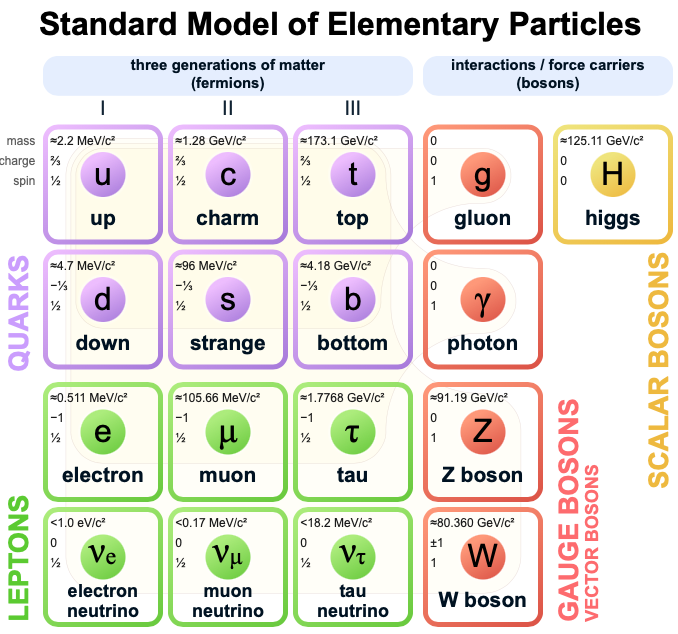
\includegraphics[width=0.8\textwidth]{Images/Theory/SMpart.png}
    \caption[Particles in the SM]{Elementary particles of the Standard Model \cite{tableSMWiki}. Elementary fermions (quarks and leptons) are listed in the three left columns representing the three generations, and elementary bosons in the two right ones, with the gauge bosons in the first column and the Higgs scalar boson in the last one. The mass, electrical charge, and spins of the particles are also reported.}
    \label{particlesSM}
\end{figure}

Particles are separated based on their intrinsic angular momentum or \textit{spin}, with half-spin particles following the Fermi-Dirac statistics constituting the fermions, and integer-spin particles obeying the Bose-Einstein statistics making the bosons. The elementary fermions are split into 6 quarks and 6 leptons each paired into three generations, with only the first generation being stable. The distinction between quarks and leptons stems from the different quantum numbers categorising them. Quarks carry a fractional electromagnetic charge as well as a colour charge, making them sensitive to the strong interaction. On the contrary, leptons are colour neutral and are either electromagnetically neutral or have a charge of -1, in units of the electron charge $|e|$. The charged leptons include the electron $e^-$, the muon $\mu^-$, and the tau $\tau^-$. The neutral leptons are called neutrinos, with one neutrino $\nu_\ell$ associated per charged lepton $\ell$, e.g., the electron-neutrino $\nu_e$ for the electron $e$. In the \gls{sm}, the number of leptons of each generation throughout an interaction is a conserved number. For the quarks, the electromagnetic charge is fractional, dividing them between \textit{up}-type quarks with charge +$2/3$ consisting of the up $u$, charm $c$, and top $t$ flavours, and the \textit{down}-type quarks with charge -$1/3$ and the flavours down $d$, strange $s$, and bottom $b$. To every particle corresponds an \textit{anti}particle, with some quantum numbers changed such as the electromagnetic charge that takes the opposite sign: e.g., the antiparticle of the electron $e^-$ is the positron $e^+$. \\

The kinematics and dynamics of the fields representing the particles in the theory are expressed through a Lagrangian density $\mathcal{L}$, a spacetime discretised element of the general Lagrangian. Symmetries of the Lagrangian density play an essential role as they define conserved quantities through Noether's theorem. The construction of the \gls{sm} Lagrangian is dictated by the expression of these symmetries to satisfy the experimentally observed conserved quantities, such as the electromagnetic charge. Two types of symmetries can be considered: global ones that are valid across spacetime and local ones, the so-called \textit{gauge} symmetries. The \gls{sm} Lagrangian must satisfy the global Poincaré symmetry, encapsulating the symmetries required by Special Relativity, and a local non-Abelian $SU(3)_C \otimes SU(2)_L \otimes U(1)_Y$ gauge symmetry. Non-Abelian groups are such that their generators do not commute and constitute the backbone of Yang-Mills theories \cite{PhysRev.96.191}. The Lagrangian density of a field $\psi$ is a function of $\psi$ and its spacetime partial derivative $\partial_{\mu} \psi$, where $\mu$ indexes the time and space dimensions in the 4-vector formalism. The full \gls{sm} Lagrangian $\mathcal{L}_{\text{SM}}$ can be decomposed into 4 terms:
\begin{equation}\label{eq-SMGlobal}
    \mathcal{L}_{\text{SM}} = \mathcal{L}_{\text{EW}} + \mathcal{L}_{\text{QCD}} + \mathcal{L}_{\text{Higgs}} + \mathcal{L}_{\text{Yukawa}}.
\end{equation}
Each term encodes a different fundamental property within the unified framework of the \gls{sm}. Three of the four known interactions of nature are encapsulated in the \gls{sm}: the strong, the electromagnetic, and the weak forces. The gravitational interaction is set aside due to the weakness of its influence at subatomic scales. The mediators of the three included interactions are the gauge bosons, which are spin 1 particles with different properties arising from the nature of the interaction they exchange. The electromagnetic and weak forces have been successfully unified as a single \gls{ew} interaction, while the strong force is described by \gls{qcd}. One essential element in the \gls{sm} is the so-called \textit{Brout-Englert-Higgs interaction}, a special force through which some particles acquire mass. This interaction, summarised as \textit{Higgs}, is underpinned by the Higgs field, an excitation of which is called a Higgs boson $H$. Yukawa interactions between the Higgs field and quarks are introduced to assign masses to the latter through Yukawa couplings. The analysis presented in Chapter~\ref{chap-VH} of this thesis is dedicated to a measurement of the Higgs couplings to the $b$- and $c$-quarks. The different fundamental interactions and their theoretical modelisations are further reviewed in this chapter.

\subsection{Quantum Electrodynamics}\label{subsec-QED}
\textit{\glsreset{qed}\gls{qed}} is the theory underpinning the behaviour of free fermions and the electromagnetic interactions, for which the gauge carrier is the photon $\gamma$. Fermions are represented by a Dirac spinor field $\psi(x)$ defined over spacetime $x$. The Dirac equation of quantum mechanics is a first-order partial derivative equation modelling the free dynamics of such a spin-$1/2$ fermion with
\begin{equation}\label{eq-dirac}
    (i\gamma^{\mu} \partial_{\mu} - m) \psi(x) = 0,
\end{equation}
where $\gamma^{\mu}$ are the Dirac $\gamma$-matrices generalising the Pauli spin matrices to spacetime dimensions $\mu$, and the Einstein notation is adopted whereby indices repeated as covariant and contravariant are summed over. For conciseness, any contraction $\gamma^{\mu} O_{\mu}$ of the $\gamma$-matrices with a 4-vector object $O$ is denoted as $\cancel{O}$. The following Lagrangian density is constructed to lead - after application of Euler-Lagrange - to the dynamics of Equation \ref{eq-dirac}:
\begin{equation}\label{eq-diracLag}
   \mathcal{L}_{\text{Dirac}} = \bar{\psi} (i \cancel{\partial}- m) \psi,
\end{equation}
where the dependency on the spacetime coordinate $x$ is henceforth omitted for clarity. Such a Lagrangian models the free dynamics of any fermion, such as an electron $e^-$ or a $c$-quark. The electromagnetic charge $q$ of particles is conserved by every known interaction. Per Noether's theorem, this conservation must in turn result from a symmetry, leading the Dirac Lagrangian to be made invariant under a local gauge $U(1)$ transformation
\begin{equation}\label{eq-GaugeU1}
    \psi(x) \rightarrow \psi'(x') = e^{-iq\alpha(x)} \psi(x),
\end{equation}
which corresponds to a rotation in the complex spacetime by a phase $q\alpha(x)$. For the Lagrangian of Equation \ref{eq-diracLag} to satisfy this symmetry, the partial derivative $\partial_{\mu}$ must be replaced by the \textit{gauge covariant derivative $D_{\mu}$}
\begin{equation}\label{eq-CoDerU1}
    D_{\mu} = \partial_{\mu} + iqA_{\mu},
\end{equation}
where a new vector field $A_{\mu}$ is introduced and required to transform under the $U(1)$ symmetry as $A_{\mu} \rightarrow A'_{\mu} = A_{\mu} + \partial_{\mu} \alpha(x)$. The elegance of this approach is the possibility to give the gauge field $A_{\mu}$ its own dynamics, modifying the Lagrangian of Equation \ref{eq-diracLag} into the \gls{qed} Lagrangian \[ \mathcal{L}_{\text{QED}} = \bar{\psi} (i \cancel{\partial}- m) \psi + q \bar{\psi} \cancel{A} \psi - \frac{1}{4} F_{\mu\nu} F^{\mu\nu}, \]
\begin{equation}\label{eq-QEDLag}
    \mathcal{L}_{\text{QED}} = \bar{\psi} (i \cancel{D}- m) \psi - \frac{1}{4} F_{\mu\nu} F^{\mu\nu},
\end{equation}
where $F_{\mu\nu} = \partial_{\mu} A_\nu - \partial_\nu A_{\mu} $ is the electromagnetic field tensor. The $F_{\mu\nu} F^{\mu\nu}$ part in Equation \ref{eq-QEDLag} introduces a kinetic term for the gauge field. The interaction between the fermion $\psi$ and the gauge field $A$ is represented by the term $q \bar{\psi} \cancel{A} \psi$, combining them with the coupling $q$. The strength of electromagnetism is defined in scale by the charge $e$ of an electron. In the present case, the electromagnetic charge $q$ is the conserved quantity of the gauge symmetry, which requires the introduction of a gauge field $A_\mu$ that is interpreted as the photon field. The Lagrangian is adapted to include the full dynamic of the electromagnetic interaction through the strength tensor $F_{\mu\nu}$. Fermionic fields are introduced with this approach for the different known fermions, $\psi_e$, $\psi_{\mu}$, $\psi_u$, $\psi_c$, etc. Their interaction with $A_\mu$ defines each time a unique conserved electromagnetic charge $q_e$, $q_{\mu}$, $q_u$, $q_c$, etc. This procedure is general: the gauge invariance of a Lagrangian introduces a spin-1 gauge boson. Interestingly, the required $U(1)$ invariance forbids the presence of mass terms of the form $m^2 A^{\mu} A_{\mu}$ in the Lagrangian, seemingly condemning gauge bosons to remain massless. 

\subsection{Electroweak Sector}
The weak force is propagated by two massive gauge vector bosons: the $W^{\pm}$, of mass $m_W \approx 80.36$ GeV\footnote{The unit system adopted throughout this thesis is to set the speed of light in vacuum $c$ at 1, leading to masses expressed in GeV. To convert to mass units, one simply needs to adopt SI units and divide by $c^2$.}, and the $Z^0$, of mass $m_Z \approx 91.19$ GeV \cite{Tanabashi:2018oca}. This apparent contradiction with the massless requirements of a $U(1)$ symmetry is elegantly solved by the Brout-Englert-Higgs mechanism \cite{Englert:1964et, PhysRevLett.13.508}. This mechanism, described in the next section, is applied to a unified expression of the electromagnetic and weak interactions known as the \textit{\glsreset{ew}\gls{ew}} interaction in the Glashow-Weinberg-Salam (GSM) model \cite{GLASHOW1961579, PhysRevLett.19.1264, Salam:1968rm}. The fundamental symmetry group the theory is built upon is the non-Abelian $SU(2)_L \otimes U(1)_Y$, where $SU(2)_L$ is the weak isospin and $U(1)_Y$ the weak hypercharge. The local $SU(2)$ transformation acts as
\begin{equation}\label{eq-GaugeSU2}
    \psi \rightarrow \psi' = e^{i g \alpha^a(x) T^a } \psi,
\end{equation}
where $T^a = \sigma^a / 2$ are the generators of the $SU(2)_L$ group, built from the $\sigma^a$ Pauli matrices ($a = 1, 2, 3)$. Each generator corresponds to a gauge field. Since these generators do not commute, the \gls{ew} sector is built on a non-Abelian group and is, therefore, a Yang-Mills theory with self-interacting gauge mediators \cite{PhysRev.96.191}. The gauge fields linked to $SU(2)_L$ lead to a covariant derivative, similarly to \gls{qed}, to ensure the invariance of the Lagrangian under the symmetry. It is expressed as
\begin{equation}\label{eq-CovDerSU2}
   D_{\mu}  = \partial_{\mu} + igT_a W_{\mu}^a,
\end{equation}
with three gauge fields $W_{\mu}^1$, $W_{\mu}^2$, $W_{\mu}^3$ and a unique interaction strength $g$. The particularity of the weak interaction is that the so-called charged current interactions that are described by the symmetry group $SU(2)_L$ only apply to left-handed ($L$) particle states and not the right-handed ($R$) states. Consequently, the fermionic fields are decomposed into \[\psi = \psi_L + \psi_R\] with left- and right-handed particles represented by isospin doublets. The weak isospin $I_W$ charge of left-handed particles is $I_W = 1/2$, with a third component $I_W^3 = \pm  1/2$. For the right-handed part, $I_W = 0$ with $I_W^3 = 0$, decoupling it from the gauge bosons $W_{\mu}^a$. Physically, the observed weak charged current interactions correspond to the $W^{\pm}$ bosons resulting from a linear combination of the first two gauge fields
\begin{equation}\label{eq-weak-lic}
    W_{\mu}^{\pm} = \frac{1}{\sqrt{2}} \left(W_{\mu}^{1} \mp W_{\mu}^{2} \right).
\end{equation}
The $W^{\pm}$ bosons are electromagnetically charged and only couple to left-handed particles, but the experimentally observed electromagnetically neutral $Z$ boson couples to both left- and right-handed particles. In the \gls{sm}, this is represented by the additional $U(1)_Y$ symmetry of the weak interaction, the weak hypercharge $Y$ with coupling $g'$, and an additional gauge field $B_{\mu}$. The weak hypercharge is set as $Y = 2 (Q - I_W^3)$ so that the electromagnetic charge $Q$ matches observations. The complete covariant derivative of the electroweak sector of the \gls{sm} is therefore expressed in the GSM model as 
\begin{equation}\label{eq-GaugeEW}
    D_{\mu}  = \partial_{\mu} + ig \frac{\sigma_a}{2} W_{\mu}^a + ig' \frac{Y}{2} B_{\mu}
\end{equation}
where $W_{\mu}^a$ and $B_{\mu}$ are respectively the $SU(2)_L$ and $U(1)_Y$ gauge bosons. The full \gls{ew} Lagrangian built with this covariant derivative is
\begin{equation}\label{eq-EWlag}
    \begin{split}
        \mathcal{L}_{\text{EW}} = - \frac{1}{4} W_a^{\mu\nu} W^a_{\mu\nu} &- \frac{1}{4} B_a^{\mu\nu} B^a_{\mu\nu} + \sum_{j} \left[ \bar{\ell}_{L_j}i\cancel{D}\ell_{L_j} + \bar{e}_{R_j}i\cancel{D}e_{r_j}  \right] \\
        &+ \sum_{j} \left[ \bar{Q}_{L_j}i\cancel{D}Q_{L_j} + \bar{u}_{R_j}i\cancel{D}u_{R_j} + \bar{d}_{R_j}i\cancel{D}d_{R_j} \right],
    \end{split}
\end{equation}
where the $W_a^{\mu\nu}$ and $B_a^{\mu\nu}$ matrices are the electroweak field strength tensors. The sum over $j$ represents the three fermionic generations, each introduced separately for the lepton fields, with the left-handed doublet $\ell$ and the right-handed singlet $e$ for the charged lepton, and the quark fields, with $Q$ representing the left-handed doublet and $u_R$ and $d_R$ the right-handed up- and down-type singlets. Neutrinos, that are in the left-handed $\ell$ doublet, only interact through the weak force. \\

The linear combination of Equation \ref{eq-weak-lic} is required to represent the physical charged fields $W^{\pm}$. Similarly, the physically observed electromagnetic photonic field $A_{\mu}$ and the $Z$ boson field $Z_{\mu}$ are the result of a linear combination of the neutral $B_{\mu}$ and $W_{\mu}^3$. This combination depends on a fundamental parameter of the \gls{sm} called the \textit{weak mixing angle} $\theta_W$ such that
\begin{equation}\label{eq-weakmixangle}
    \cos\theta_W = \frac{g}{\sqrt{g^2 +g'^2}},
\end{equation}
thereby establishing a connection between the coupling strengths of the weak interaction and the electromagnetic interaction as \[e = g \sin \theta_W = g' \cos\theta_W.\] The intrinsic strength of the weak interactions is of similar order to that of the electromagnetic interaction but is weak in appearance due to the large mass of its gauge vector bosons. The weak force is the only known fundamental interaction to violate symmetry under parity transformation. A significant achievement of modern particle physics is the unification of interactions that are perceived as different at low energies. The problem of the mass of the gauge bosons however remains. Additionally, the split of fermionic fields into left- and right-handed components leads fermionic mass terms in the \gls{qed} Lagrangian of Equation~\ref{eq-QEDLag} to violate the gauge invariance. Both issues are resolved by considering an additional scalar field, following the Brout-Englert-Higgs mechanism, and introducing Yukawa interactions, as explained in the next sections.

\subsection{The Brout-Englert-Higgs Mechanism}
The \textit{Brout-Englert-Higgs mechanism (BEH)} offers an elegant solution to introduce mass terms for the gauge fields $W_{\mu}^{\pm}$ and $Z_{\mu}$ \cite{Englert:1964et,  PhysRevLett.13.508}. It postulates the existence of an additional scalar Higgs field permeating the Universe. The field is mathematically defined as a weak isospin doublet, with a neutral component $\phi^0$ and a charged one $\phi^+$. They are jointly expressed as a complex scalar field $\phi$ with 4 degrees of freedom
\begin{equation}
\phi = \begin{pmatrix}
    \phi^+\\ 
    \phi^0
\end{pmatrix} = \frac{1}{2} \begin{pmatrix}
    \phi_1 + i\phi_2 \\ 
    \phi_3 + i\phi_4
\end{pmatrix}.
\end{equation}
This complex scalar field interacts with the electroweak gauge fields through the covariant derivatives of Equation~\ref{eq-GaugeEW} as 
\begin{equation}\label{eq-HiggsLag}
    \mathcal{L_{\text{Higgs}}} = (D_{\mu}\phi)^{\dagger} (D^{\mu}\phi) - V(\phi),
 \end{equation}
where the first term describes the kinetic energy of the $\phi$ field and the second term is the Higgs potential energy
\begin{equation}\label{eq-HiggsPot}
 V(\phi) = - \mu^2  \phi^{\dagger} \phi + \lambda (\phi^{\dagger} \phi)^2.
\end{equation}
The expression of this potential is constrained by the need for the theory to be renormalisable. Two scalar constants govern the Higgs potential: $\mu$ and $\lambda$ describing, respectively, the quadratic and quartic interactions of the complex Higgs field $\phi$. The former manifests the interaction with the electroweak gauge bosons, while the latter introduces Higgs self-interactions. The minimum of this potential corresponds to the vacuum state. The requirement that the vacuum be stable demands $\lambda > 0$. For a positive $\mu^2 > 0$, a degenerate minimum is found at non-null field values such that
\begin{equation}\label{eq-HiggsVacEq}
    \phi^{\dagger} \phi  = \frac{1}{2} (\phi_1^2 + \phi_2^2 + \phi_3^2 + \phi_4^2) = \frac{\mu^2}{2\lambda} = \frac{v^2}{2}
\end{equation}
introducing in the last equality the so-called \textit{vacuum expectation value} $v = \sqrt{\frac{\mu^2}{\lambda}}$ of the field $\phi$. The infinite degeneracy of the Higgs potential vacuum states underlines a special $SU(2)$ symmetry such that $\phi^{\dagger} \phi = v^2/2$. Through \textit{spontaneous symmetry breaking}, the BEH mechanism crumbles this degeneracy into one single vacuum state, typically chosen by setting the components $\phi_1 = \phi_2 = \phi_4 = 0$ and $\phi_3 = v$ so that the vacuum expectation is simply
\begin{equation}
\langle 0|\phi|0 \rangle = \frac{1}{\sqrt{2}} \begin{pmatrix}
        0\\ 
        v
    \end{pmatrix}.
\end{equation}
The breaking of the symmetry enforces $SU(2)_L \otimes U(1)_Y \rightarrow U(1)_Q$, preserving the electromagnetic symmmetry with the vacuum state correctly set as chargeless \cite{DJOUADI20081}. To model the full field dynamics around the chosen vacuum state, the particular \textit{unitarity gauge} \cite{PhysRevD.7.1068} choice is adopted to absorb unphysical Goldstone bosonic fields \cite{Goldstone:343400}, simplifying the expansion to
\begin{equation}
    \phi(x) = \frac{1}{\sqrt{2}} \begin{pmatrix}
            0\\ 
            v + h(x)
        \end{pmatrix},
\end{equation}
where $h$ is the neutral Higgs real scalar field. Introducing this expression into the Higgs Lagrangian of Equation~\ref{eq-HiggsLag} gives
\begin{equation}\label{eq-fullHiggs}
    \begin{split}
        \mathcal{L}_{\text{Higgs}} = & \,\frac{1}{2} (\partial_\mu h)(\partial^\mu h) + \frac{\mu^2}{2}(v+h)^2  - \frac{\lambda}{16}(v+h)^4 \\
        &+ v^2 \frac{g^2}{4} (W_{\mu}^+W^{\mu-})(1+\frac{h}{v})^2 + v^2 \frac{g^2 + {g'}^2}{8}(Z_{\mu}Z^{\mu})(1+\frac{h}{v})^2, 
    \end{split}
\end{equation}
where mass terms appear for the physical gauge fields $W_{\mu}^{\pm}$ and $Z_\mu$ in the last line, but not for $A_{\mu}$ as required from observations that photons are massless. The masses of the gauge vector bosons are
\begin{equation}
    m_W = \frac{v}{2} g , \quad m_Z = \frac{v}{2}\sqrt{g^2 +g'^2} 
\end{equation}
or equivalenty expressing the mass of the $W$ boson in terms of the $Z$ boson mass and weak mixing angle $\theta_W$ \[m_W = m_Z \cos\theta_W.\] The Higgs field is massive with mass \[m_H = \sqrt{2\mu^2}.\] The BEH mechanism elegantly assigns mass to the gauge vector bosons while leaving the photon massless. It requires the addition of the scalar Higgs boson $H$ as a massive spin-1 elementary particle. Furthermore, the introduction of the Higgs field permits the expression of mass terms for the fermions in the \gls{sm}, as explained in Section~\ref{subset-yukint} on Yukawa interactions. 

\subsection{Quantum Chromodynamics}
The strong interaction is described by the theory of \textit{\glsreset{qcd}\gls{qcd}} underpinned by an $SU(3)_C$ symmetry with a conserved quantum number called \textit{colour}. The only particles having a colour charge in the \gls{sm} are quarks and the gauge mediators of the strong interaction: the gluons $g$. There are three colour charges typically labelled \textit{red}, \textit{blue}, and \textit{green}, each coming with anticolour, e.g., red and antired. Quarks carry one such charge. Similarly to the electroweak sector, the symmetry leads to a covariant derivative under the $SU(3)_C$ group of
\begin{equation}\label{eq-GaugeQCD}
    D_{\mu}  = \partial_{\mu} + ig_s \frac{\lambda_a}{2} G_{\mu}^a
\end{equation}
where the coupling constant $g_s$ of the strong interaction is often re-expressed as $\alpha_s = \frac{g_s}{4\pi}$, and the generator of the $SU(3)_C$ group are built with the set of $\lambda_a$ Gell-Mann matrices. The gauge fields introduced here are the $G_{\mu}^a$ corresponding to the gluonic mediators of the strong field. Gluons carry 2 colour charges, leading to the 8 Gell-Mann matrices $\lambda^a$ and 8 gauge vector fields $G_{\mu}^a$, indexed by $a$. The generators of the $SU(3)_C$ group do not commute since \[ [\lambda^a, \lambda^b] = i f^{abc} \lambda^c,\] where $f^{abc}$ are the $SU(3)_C$ structure constants. The non-commutation of the $SU(3)_C$ generators means the $SU(3)_C$ part of the \gls{sm} is a non-Abelian group, and therefore a case of a Yang-Mills theory with self-interacting gauge fields \cite{PhysRev.96.191}. Gluonic strength tensors are built similarly to the electromagnetic strength tensor as \[G_{\mu\nu}^a = \partial_{\mu} G_{\nu}^a   - \partial_{\nu} G_{\mu}^a - g_s f^{abc} G_{\mu}^b G_{\nu}^c,\] with the structure constants generating self-interactions. \\

The full \gls{qcd} Lagrangian is
\begin{equation}\label{eq-QCDLag}
    \mathcal{L}_{\text{QCD}} = -\frac{1}{4} G_{\mu\nu}^a G^{\mu\nu}_a + \sum_{f} \bar{\psi}_f (i \cancel{D} - m_f) \psi_f,
\end{equation}
where $\psi_f$ are the six quarks fields, one per flavour $f$, transforming as an $SU(3)_C$ triplet with one component per colour quantum number. \\

Like every coupling constant, $\alpha_s$ varies with energy. At low energies, the interaction is so strong that perturbative calculations break and the behaviour of \textit{colour confinement} is observed: any attempt to isolate a quark requires such a large amount of energy that a quark-antiquark pair is spontaneously produced. The shear strength of this interaction explains its short propagation distance despite the fact its gluonic mediators are massless. At higher energies, asymptotic freedom and perturbative calculations are possible thanks to the reduced coupling strength. This typically requires higher-order corrections for the calculation to converge, with some terms, such as quark self-energy loops, diverging to infinity. These so-called \textit{ultraviolet divergences} are removed by renormalising fields and parameters so that the infinities are absorbed away. This correction requires two parameters to arbitrarily define the scale of the process: the \textit{renormalisation scale} $\mu_R$ and \textit{factorisation scale} $\mu_F$ \cite{collins2004factorization}. The former is introduced to deal with the ultraviolet divergences in the running of $\alpha_s$. The latter addresses the so-called \textit{infrared divergences} due to massless particles radiating further massless particles at low energies, and enters the parton distribution and fragmentation functions introduced later in this chapter.\\

Quarks combine to form colourless aggregates of matter called \textit{hadrons}, with either a di-quark system combining a quark and an antiquark into a \textit{meson}, or a tri-quark system forming a \textit{baryon} of which the proton $p$ ($uud$, $q_p = +1$) and the neutron $n$ ($udd$, $q_n = 0$) are prime examples. The particles constituting the hadrons are called partons. The process leading to the neutralisation of the colour charge of an asymptotically free quark is called \textit{hadronisation}.

\subsection{Yukawa Interactions}\label{subset-yukint}
In the \gls{qcd} Lagrangian of Equation~\ref{eq-QCDLag}, the introduction of mass terms for the quarks breaks the gauge invariance of the theory under $SU(2)_L \otimes U(1)_Y$, requiring $m_f = 0$. The masses of all fermions are instead included in the \gls{sm} through Yukawa interactions between the Higgs and fermionic fields \cite{10.1143/PTPS.1.1}. These terms are expressed by the following Lagrangian
\begin{equation}\label{eq-YukLag}
    \mathcal{L}_{\text{Yukawa}} = - \frac{1}{\sqrt{2}} \sum_{f} 
    y_f \bar{\psi}_f (v + h) \psi_f,
\end{equation}
where $\psi_f$ are the fermionic fields and the fundamental \textit{Yukawa couplings} $y_f = \sqrt{2}m_f/v$ are introduced as coupling strengths for each flavour of electrically charged fermion $f$. Picking the $v$ components in the sum in parentheses gives mass terms $m_f$ to the fermions, with the $h$ terms leading to Higgs-fermion interactions proportional to the fermion mass. The vacuum expectation value plays the role of a general mass scale of the theory, with Yukawa couplings refining the specific mass of each fermionic species. \\

For the quark sector, a further correction is required as the weak interaction eigenstate basis is different from the mass basis in which physical particles are detected. The transformation from the mass eigenstates basis is specified by the complex unitary \textit{\gls{ckm} matrix} \cite{Tanabashi:2018oca}
\begin{equation}
    V_{CKM} = \begin{pmatrix}
            V_{ud} & V_{us} & V_{ub}\\ 
            V_{cd} & V_{cs} & V_{cb}\\ 
            V_{td} & V_{ts} & V_{tb}\\ 
        \end{pmatrix},
\end{equation}
where the probability of a transition $p \rightarrow q$ is given by the magnitude $|V_{pq}|^2$ of the associated element. Through this quark mixing matrix, weak-charged current interactions allow for flavour-changing processes. The matrix is almost diagonal in magnitude, hence transitions between quarks of the same generation are preferred: e.g., $t \rightarrow b$ is favoured over $t \rightarrow d$.

\section{Experimental Higgs Phenomenology}\label{th-sec-higphe}
The experimental process to observe the Higgs bosons at the \gls{lhc} is to collide two proton beams head-on, as described in Chapter~\ref{chapter-ATLAS}. Protons are composite particles and, at high energies, the main \textit{hard-scattering} interaction is between components of the protons called the \textit{partons}. These partons consist of the \textit{valence} quarks ($uud$ for a proton) but there are also contributions from \textit{sea} quarks, as well as gluons and photons, present within the hadron due to quantum fluctuations. In a $pp$ collision, two interacting partons $a$ and $b$ from each proton undergo the main event $ab \rightarrow X$, with the activity from the rest of the protons assigned to the \textit{\gls{ue}}. The cross section for the global process $pp \rightarrow X$ is expressed using the factorisation theorem \cite{collins2004factorization} as 
\begin{equation}
\sigma_{pp\rightarrow X} = \sum_{a,b} \int_0^1 dx_a \int_0^1 dx_b f_a(x_a, \mu_F) f_b(x_b, \mu_F) \int d\sigma_{ab\rightarrow X}\left(x_aP_a, x_bP_b, \mu_R, \mu_F \right),
\end{equation}
where $f_i(x_i, \mu_F)$ is the \textit{\gls{pdf}} giving the probability for the parton $i$ to undergo a hard scattering with momentum $p_i = x_i P_i$ taken as a fraction $x_i$ of the proton momentum $P_i$, and $\mu_F$ is the previously introduced factorisation scale symbolising the dependency of the \gls{pdf} on the energy scale of the underlying process $ab \rightarrow X$. The interaction is effectively factorised into two terms: the first picking up the interacting partons and their fraction of momentum and the second considering the main $ab \rightarrow X$ event.\\

As introduced in the previous section, the Higgs $H$ couples to particles proportionally to their mass, which impacts the production and decay modes of the boson. The leading order production modes of the Higgs boson are schematised in Figure \ref{fig:prodH}. At the \gls{lhc}, with the centre-of-mass energy of $\sqrt{s} = 13$ TeV in Run 2 $pp$ collisions and a Higgs boson mass $m_H = 125$ GeV, the main processes are, by decreasing cross section: 
\begin{itemize}[leftmargin=*]
    \item \textit{Gluon-gluon fusion ($ggF$)}: two partonic gluons fuse into a quark loop with a radiated Higgs boson as $pp \rightarrow H$. The quarks in the loop couple to the Higgs, hence the massive top $t$-quarks are preferred, followed by bottom $b$-quarks. The cross section for this process is $\sigma_{ggF} = 48.6 \pm 2.4$ pb \cite{LHCHiggsCrossSectionWorkingGroup:2016ypw}. This process is favoured thanks to the large contributions of gluons to the protonic \gls{pdf}s at the energies considered.
    \item \textit{Vector boson fusion ($VBF$)}: two off-shell vector bosons $V$ ($W$ or $Z$) radiated from partonic quarks fuse to form a Higgs as $pp \rightarrow qqH$, with cross section $\sigma_{VBF} = 3.77 \pm 0.09$ pb \cite{LHCHiggsCrossSectionWorkingGroup:2016ypw}. The quarks leave the characteristic signature of a forward jets pair in the event.
    \item \textit{Associated production with a vector boson ($VH$)}: the Higgs boson is produced in association with a vector boson $V$ as $pp \rightarrow VH$, with a cross section of $\sigma_{VH} = 2.24 \pm 0.14$ pb \cite{LHCHiggsCrossSectionWorkingGroup:2016ypw}. This process is studied in detail in Chapter~\ref{chap-VH}, through an analysis of Higgs bosons decaying to pairs of $b$- or $c$-quarks in this $VH$ production mode. Experimentally, requiring leptonic decays of the associated vector boson gives a clean event signature.
    \item \textit{Associated production with a quark pair ($q\bar{q}H$)}: an open quark loop is produced from a pair of partonic gluons, with a Higgs radiated as $pp \rightarrow q\bar{q}H$. The dominating contributions come from the $t\bar{t}H$ associated production with cross section $\sigma_{VH} = 0.51 \pm 0.04$ pb, followed by the $b\bar{b}H$ \cite{LHCHiggsCrossSectionWorkingGroup:2016ypw}.
\end{itemize}

\begin{figure}[h!]
    \center
    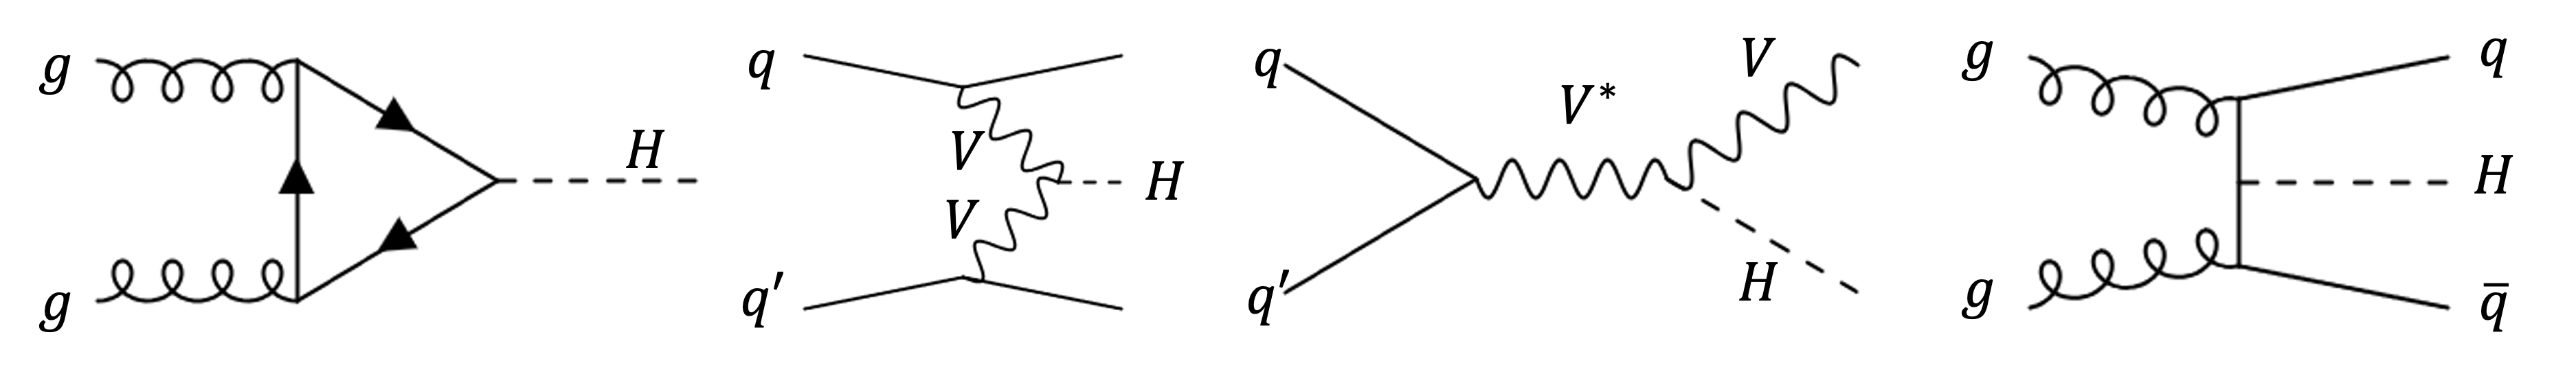
\includegraphics[width=\textwidth]{Images/Theory/higgsprod.png}
    \caption{The leading order Feynman diagrams for Higgs production at the LHC, from left to right: gluon-gluon fusion, vector boson $V$ fusion, vector boson associated production, and $q\bar{q}$ associated production.}
    \label{fig:prodH}
\end{figure}

The cross section dependency of the Higgs boson production modes from proton-proton collisions at $\sqrt{s} = 13$ TeV are represented in the left of Figure~\ref{fig:prodHcross} as a function of the Higgs boson mass $m_H$. The total width of the \gls{sm} Higgs boson with $m_H = 125$ GeV is $\Gamma_H = 4$ MeV, implying a short lifetime of $\tau_H \sim10^{-22}$~s limiting direct measurements to the decay products. The branching ratios at $\sqrt{s} = 13$ TeV are displayed on the right of Figure~\ref{fig:prodHcross}, with decays to heavier particles favoured due to the proportionality of the Higgs coupling strength to the mass. Decays to the massless gluons $g$ and photons $\gamma$ are possible thanks to intermediate quark loops, similarly to $ggF$. Relative decay rates are quantified by their branching ratio $BR$ as
\begin{equation}
    BR (H \rightarrow X) = \frac{\Gamma (H\rightarrow X)}{\Gamma_H},
\end{equation}
where the total Higgs width $\Gamma_H$ is the sum of all partial decay width $\Gamma (H\rightarrow X)$, for all possible $X$. The most likely Higgs decay mode is to a $b\bar{b}$ pair ($\sim58$\%), followed by the decay to a $WW$ pair ($\sim21$\%). The $c\bar{c}$ decay branching ratio is $\sim2.9$\%. \\

\begin{figure}[h!]
    \center
    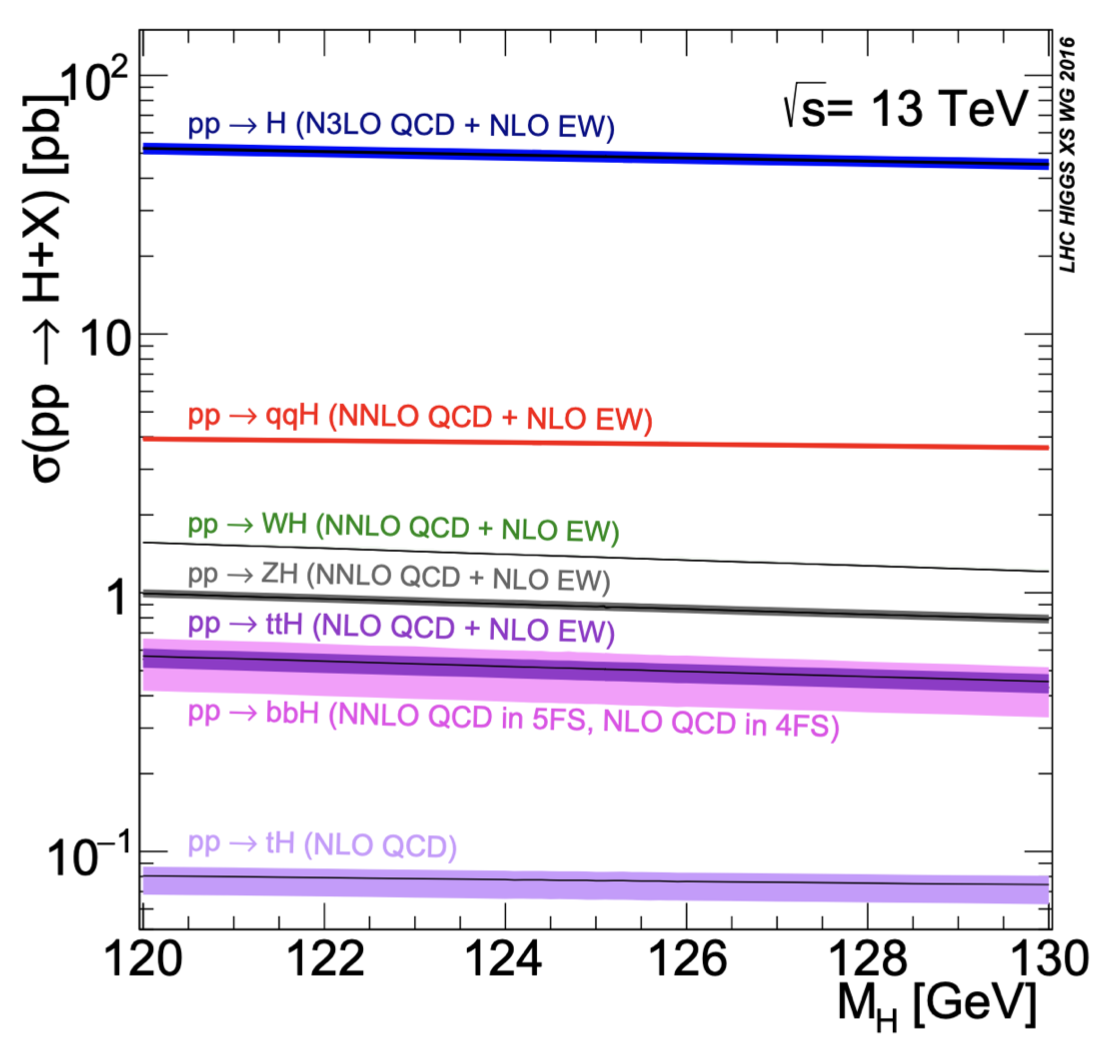
\includegraphics[width=0.48\textwidth]{Images/Theory/prodHiggs.png}
    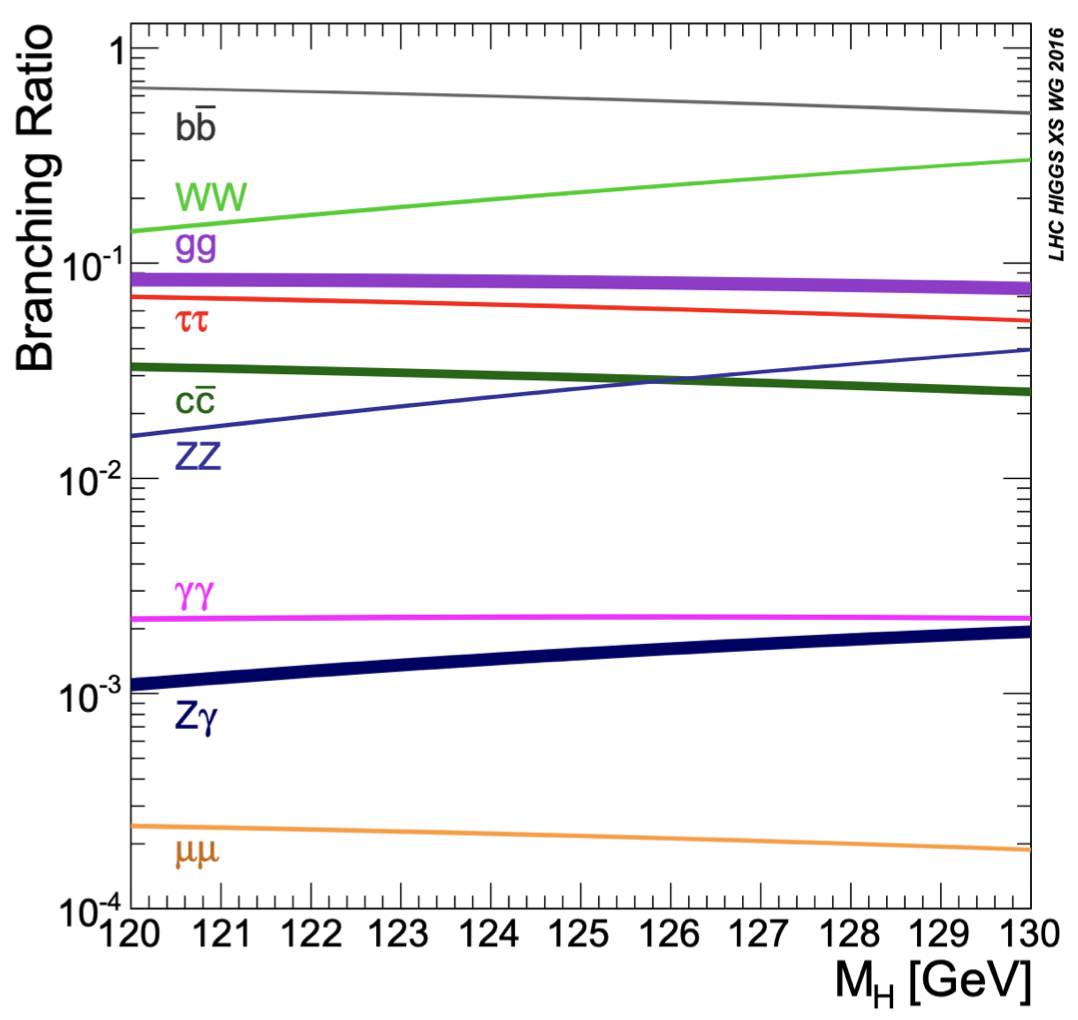
\includegraphics[width=0.48\textwidth]{Images/Theory/decayHiggs.png}
    \caption{The Standard Model production cross sections from proton-proton collisions (left) and decay branching ratio (right) of the Higgs boson as a function of $m_H$ at $\sqrt{s} = 13$ TeV \cite{LHCHiggsCrossSectionWorkingGroup:2016ypw}.}
    \label{fig:prodHcross}
\end{figure}
\begin{figure}[h!]
    \hspace{-0.48cm}
    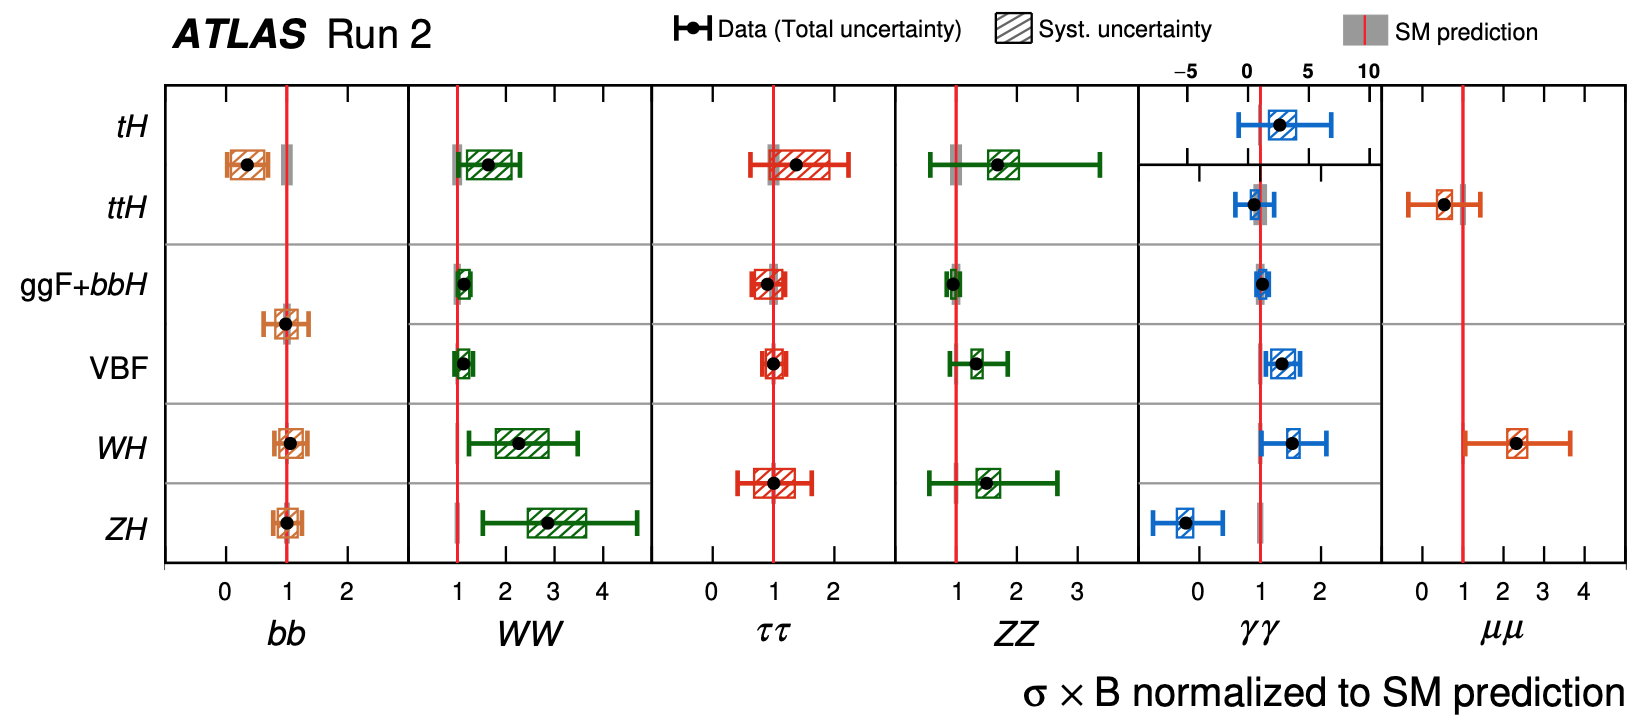
\includegraphics[width=\textwidth]{Images/Theory/allMesRun2.png}
    \caption{Ratio of observed signal strengths to the SM predictions for different combinations of Higgs boson production and decay modes \cite{ATLAS:2022vkf}. Horizontal bars denote the 68\% confidence interval, with grey bands showing theory uncertainties on the SM cross section $\times$ branching ratio predictions.}
    \label{fig:measprodH}
\end{figure}

The $WW$ and $ZZ$ decays can only be achieved via virtual off-shell Higgs bosons, reducing their contributions despite their large mass. Fermionic decays are challenging to observe in hadron colliders due to the large multi-jet background. The vector bosons and di-photon leptonic decays benefit from advantageous experimental conditions, being easier to identify thanks to the presence of leptons and suffering from less background contamination. For these reasons, the ATLAS and CMS Collaborations observed in 2012 a particle of mass $m_H = 125$ GeV with the properties of the Higgs boson by combining searches for $H \rightarrow \gamma\gamma$, $H \rightarrow ZZ \rightarrow \ell^+\ell^-\ell'^+\ell'^-$, and $H \rightarrow W^+W^- \rightarrow \ell^+\ell^-\nu \bar{\nu}$ \cite{ATLAS:2012yve, CMS:2012qbp}. This paved the way for many additional Higgs measurements, summarised in Figure \ref{fig:measprodH}. Decay modes to the electroweak gauge bosons and third-generation fermions ($t, b, \tau$) have all been observed, and the sensitivity to the second generation ($\mu$) is approaching evidence level. The observed Higgs boson is remarkably consistent with the \gls{sm} predictions \cite{ATLAS:2022vkf}. 